
\chapter{Theory}

\section{Standard model}

Standard model(SM) describes the properties of the fundamental particles currently known in the universe and the interactions amount them.  The discovery of Higgs boson in 2012 implement the last missing piece in SM.  The particles in SM is shown in Figure.~\ref{fig:SM_particles}. Besides Higgs boson, there are three generations of leptons and quarks and four gauge bosons. 
Leptons and quarks are fermions that compose the matters currently known in the universe, while the gauge bosons serve as the mediators of interactions.  

SM is a gauge theory, which describes three natural force, the strong, electromagnetic and weak force by symmetry group $SU(3)_{C}\times SU(2)_{L}\times U(1)_{Y}$. Electroweak section is described by $SU(2)_{L}\times U(1)_{Y}$. The L in $SU(2)_{L}$ stands for the left chiral signature of the weak interaction and the Y in $U(1)_{Y}$ stands for the weak hypercharge. Strong interaction is described by $SU(3)_{C}$, in which the C stands for the colors of quarks.  Photons, gluons and $W^{\pm}$, Z bosons are the mediators of electromagnetic, strong and weak force respectively.  Gravity force is not included in SM. Each particles in Figure.~\ref{fig:SM_particles} has its anti-particle or the anti-particle is the particle itself. The force and mediators characters are summarized in Table.~\ref{Mediator_infor}

\begin{figure}[htbp] 
\centering
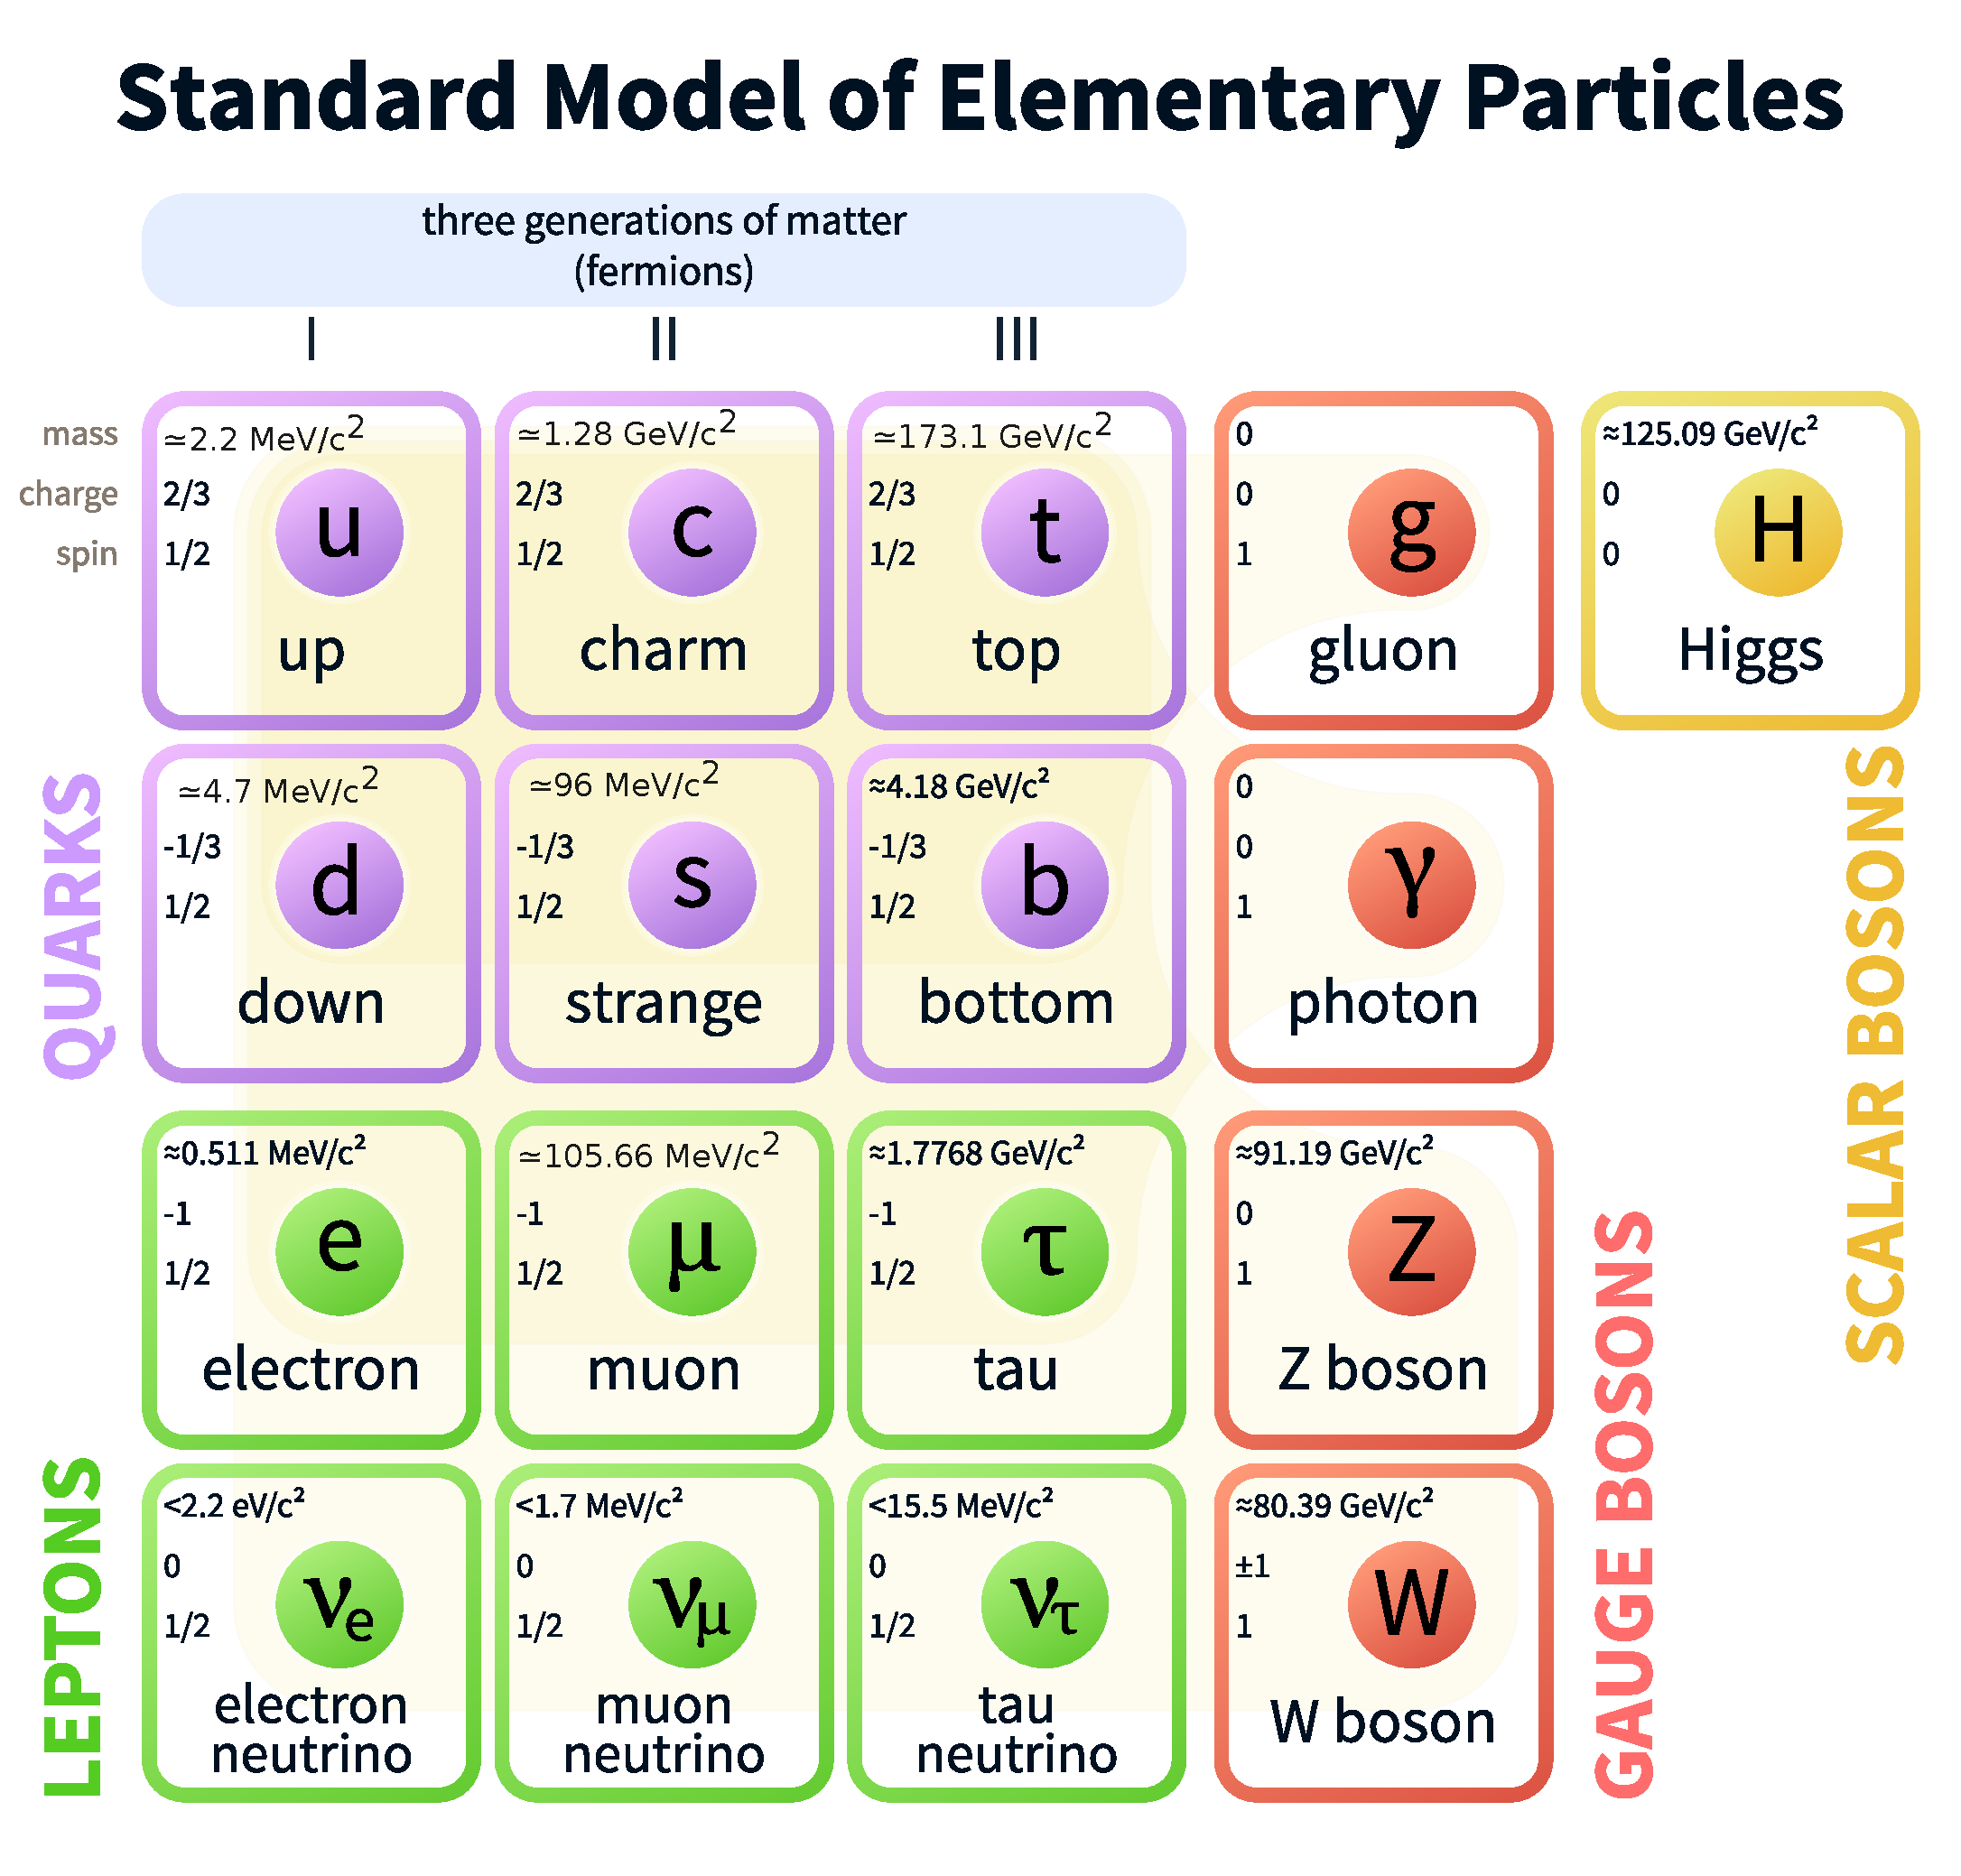
\includegraphics[width=0.8\textwidth]{chapter2/SM_particle_table.pdf}
\caption{Standard model particle group\cite{SM_particletable}}
\label{fig:SM_particles}
\end{figure}


\begin{table}[htp]
\caption{Mediators in standard model~\cite{Griffiths:111880}}
\begin{center}
\begin{tabular}{|c|c|c|c|c|}
\hline
Force & Mediator & Charge & Mass(GeV) & Range(m)   \\\hline
Strong                & g(8 gluons)                  & 0 & 0 & $10^{-15}$   \\\hline
Electromagnetic & $\gamma$(photon)     & 0 & 0 &   $\infty$   \\\hline
Weak                  &  $W^{\pm}$                &$\pm$1 & 80.379 &$10^{-18}$\\
                           & Z                                &  0         & 91.1876 &  $10^{-18}$ \\\hline
\end{tabular}
\end{center}
\label{Mediator_infor}
\end{table}%


Fermion fields in SM can be further categorized. In weak interaction, left-handed fermions are isodoublets, while right-handed fermions are isosinglets. Only the left-handed fermions or right-handed anti-fermions participate in the weak interaction. Weak hypercharge is a combined quantity, which is defined by the electric charge Q the third component of the weak isospin $I^{3}_{f}$, $Y=Q-I^{3}_{f}$. Weak interaction, together with Electromagnetic interaction are best described and understood by the electro-weak theory, which is be further discussed in the next section.  Quarks are described by SU(3), which are color triplets, while leptons are color singlets.   

Mediators in the interaction are represented by the gauge boson fields. $B_{\mu}$ is associated with symmetry $U(1)_{Y}$ and the corresponds generator is Y. $W_{\mu}^{1,2,3}$ are associated to $SU(2)_{L}$ symmetry with the generator $T^{a}$(a=1,2,3). $T^{a}$ are the $2\times2$ Pauli matrices. $G_{\mu}^{1...,8}$ are associated with the $SU(3)_{c}$ symmetry and the corresponding generators are the Gell-Mann matrices.  The field strengths are expressed as 
\begin{equation}
  \begin{aligned}
G^{a}_{\mu v}&=\partial_{\mu}G^{a}_{v}-\partial_{v}G^{a}_{\mu}+g_{s}f^{abc}G^{b}_{\mu}G^{c}_{v}\\
W^{a}_{\mu v}&=\partial_{\mu}W^{a}_{v}-\partial_{v}W^{a}_{\mu}+g_{2}\epsilon^{abc}W^{b}_{\mu}W^{c}_{v}\\
B_{\mu v}       &=\partial_{\mu}B_{v}-\partial_{v}B_{\mu}
  \end{aligned}
\end{equation}
The $g_{s}$ and $g_{2}$ are the coupling constant of $SU(3)_{C}$ and $SU(2)_{L}$ respectively. With the requirement of local gauge invariable, covariant derivatives are widely used. An example of covariant derivative acting on left-handed quarks in Lagrangian is expressed as
\begin{equation}
  \begin{aligned}
D_{\mu}\psi = (\partial_{\mu}-ig_{s}T_{a}G^{a}_{\mu}-ig_{2}T_{a}W^{a}_{\mu}-ig_{1}\frac{Y_{q}}{2}B_{\mu})
  \end{aligned}
\end{equation} 


The masses of the gauge bosons in weak interaction and fermions are generated by spontaneous symmetry breaking. Fermions specifically are generated by Higgs mechanism.  If mass terms are directly added in, the local $SU(2)\times U(1)$ will be destroyed~\cite{DJOUADI20081}. Local symmetry referring to the transformations on the fields are the functions that involve space-time. In SM, the interaction between fermion fields and scaler fields are through Yukawa's interaction.  The SM in $SU(3)_{C}\times SU(2)_{L}\times U(1)_{Y}$ symmetry without the mass terms and Yukawa's interactions is given by
 \begin{equation}
  \begin{aligned}
L_{SM}=&-\frac{1}{4}G^{a}_{\mu v}G^{\mu v}_{a}-\frac{1}{4}W^{a}_{\mu v}W^{\mu v}_{a}-\frac{1}{4}B_{\mu v}B^{\mu v}+\bar{L}_{i}iD_{\mu}\gamma^{\mu}L_{i}\\
              &+\bar{e}_{R_{i}}iD_{\mu}\gamma^{\mu}e_{R_{i}}+\bar{Q}_{i}iD_{\mu}\gamma^{\mu}Q_{i}+\bar{\mu}_{R_{i}}iD_{\mu}\gamma^{\mu}\mu_{R_{i}}+\bar{R_{i}}iD_{\mu}\gamma^{\mu}d_{R_{i}}
  \end{aligned}
\end{equation} 






\subsection{Spontaneous symmetry breaking and Higgs mechanism}

In SM, the electroweak sector follows the $SU(2)_{L}\times U(1)_{Y}$, which is spontaneously broken in the $SU(2)_{L}$ part. This mechanism plays an important role in giving mass to the mediator bosons in weak interaction and introducing the Higgs boson(Higgs).  Higgs is responsible for generating the mass of the fermions in SM, while SM remains renormalizable in local symmetry. A good example of showing the concept of spontaneous symmetry breaking with the $\phi^{4}$ theory can be found in~\cite{Peskin:1995ev}.

In the real case of SM, spontaneous symmetry breaking is introduced through a scalar doublet:
\[
\phi=
\begin{pmatrix}
\phi^{+}\\
\phi^{0}
\end{pmatrix}
=\frac{1}{\sqrt{2}}
\begin{pmatrix}
\phi_{2}-i\phi_{1}\\
\phi_{4}-i\phi_{3}
\end{pmatrix}
\]
The corresponding terms of the scalar doublet in the SM Lagrangian are expressed as
\begin{equation}
L_{s}=(D^{\mu}\phi)^{\dagger}(D_{\mu}\phi)-\mu^{2}\phi^{\dagger}\phi-\lambda(\phi^{\dagger}\phi)^{2}
\end{equation}
If $\mu^{2}<0$ and $\lambda>0$, the doublet field $\phi$ will have a none zero minimum value, which is called the vacuum expectation value(vev). In SM, the vev is shown in the following Equation and measured to be 246 GeV.
\begin{equation}\label{vev}
\langle 0 | \phi | 0 \rangle   =
\begin{pmatrix}
0\\
\frac{v}{\sqrt{2}}
\end{pmatrix}
~~~\textrm{with} ~~~  v=
\bigg(-\frac{\mu^{2}}{\lambda}\bigg)^{1/2}
\end{equation}

When the SU(2) symmetry is spontaneously broken, the scalar doublet field $\phi$ can expand around vev at first order together with the Higgs field:
\begin{equation}\label{Higgs_vev_expansion}
\phi=
\begin{pmatrix}
\theta_{2}+i\theta_{1} \\
\frac{1}{\sqrt{2}}(v+H)-i\theta_{3}
\end{pmatrix}
=e^{i\theta_{a}(x)T^{a}(x)/v}
\begin{pmatrix}
0\\
\frac{1}{\sqrt{2}}(v+H)
\end{pmatrix}
\end{equation}
Taking the unitary gauge, the scalar field transforms $\phi \to e^{-i\theta_{a}(x)T^{a}(x)/v}\phi$ and takes into $(D^{\mu}\phi)^{\dagger}(D_{\mu}\phi)$:
\begin{equation}\label{Lag_scaler}
\begin{aligned}
(D^{\mu}\phi)^{\dagger}(D_{\mu}\phi)=&|(\partial_{\mu}-ig_{2}\frac{T_{a}}{2}W^{a}_{\mu}-\frac{i}{2}g_{1}B_{\mu})\phi|^{2}\\
                                                          =&\frac{1}{2}(\partial_{\mu}H)^{2}+\frac{1}{8}g^{2}_{2}(v+H)^{2}|W^{1}_{\mu}+iW^{2}_{\mu}|^{2}\\
                                                            &+\frac{1}{8}(v+H)^{2}|g_{2}W^{3}_{\mu}-g_{1}B_{\mu}|^{2}
\end{aligned}
\end{equation}
To meets the experimental observations, re-groups the gauge fields to have the $W^{\pm}$ and Z bosons: 
\begin{equation}
W^{\pm}=\frac{1}{\sqrt{2}}(W_{1}\mp iW_{2}), Z_{\mu}=\frac{g_{2}W^{3}_{\mu}-g_{1}B_{\mu}}{\sqrt{g_{2}^{2}+g^{2}_{1}}},A_{\mu}=\frac{g_{2}W^{3}_{\mu}+g_{1}B_{\mu}}{\sqrt{g_{2}^{2}+g^{2}_{1}}},
\end{equation}
From the terms in Equation~\ref{Lag_scaler} that involving the mass of $W^{\pm}$ and Z boson, these vector bosons acquire the mass as
\begin{equation}
M_{W}=\frac{1}{2}vg_{2}~~~\textrm{and}~~~M_{Z}=\frac{1}{2}v\sqrt{g^{2}_{2}+g^{2}_{1}}
\end{equation}
while the photon $A_{\mu}$ remains massless. The mixing of electromagnetic and weak interaction is often expressed in terms of Weinberg angle or weak mixing angle. The angle $\theta_{W}$ is defined as following:
\[
\begin{pmatrix}
\gamma    \\
Z^{0}
\end{pmatrix}
=
\begin{pmatrix}
cos\theta_{W}  & sin\theta_{W} \\
-sin\theta_{W}  & cos\theta_{W}
\end{pmatrix}
\begin{pmatrix}
B\\
W_{3}
\end{pmatrix}
\]
\begin{equation}
M_{Z}=\frac{M_{W}}{cos\theta_{W}}~~~ \textrm{and}~~~
cos\theta_{W}=\frac{g_{2}}{\sqrt{g_{2}^{2}+g_{1}^{2}}}
\end{equation}

The mass of the fermions can also be generated with the interaction between the scalar doublet $\phi$ and fermion fields. Taking muon as an example, the interaction term in Lagrangian and the term that give mass to muon is shown as following:
\begin{equation}\label{Higgsmuonmass}
L_{\mu}=-\lambda_{\mu}(\bar{v}_{\mu},\bar{\mu}_{L})\phi\mu_{R}
            =-\frac{1}{\sqrt{2}}\lambda_{\mu}(v+H)\bar{\mu}_{L}\mu_{R}+ \cdots
\end{equation}
The mass of muon is given as $M_{\mu}=\frac{\lambda_{\mu}v}{\sqrt{2}}$ so as very similarly the mass of other fermions. The coupling of Higgs and fermions can also be derived from Equation.~\ref{Higgsmuonmass}~\cite{DJOUADI20081}. 

The Higgs boson production modes at LHC are the gluon-gluon fusion(ggH), the vector boson fusion(VBF), the associated production with a vector boson(VH) and the production in association with a pair of top quarks($t\bar{t}H$). The Feynman diagrams for these production modes are shown in Figure.~\ref{fig:SM_H_production}. In LHC, the proton proton collision, the real collisions are between quarks and gluons. The ggH holds the biggest Higgs production cross section, while the VBF follows. The other two are relatively small compared with ggH and VBF, thus, these two main production modes are the ones considered in the analysis that talked in the later chapters.   
\begin{figure}[htbp] 
\centering
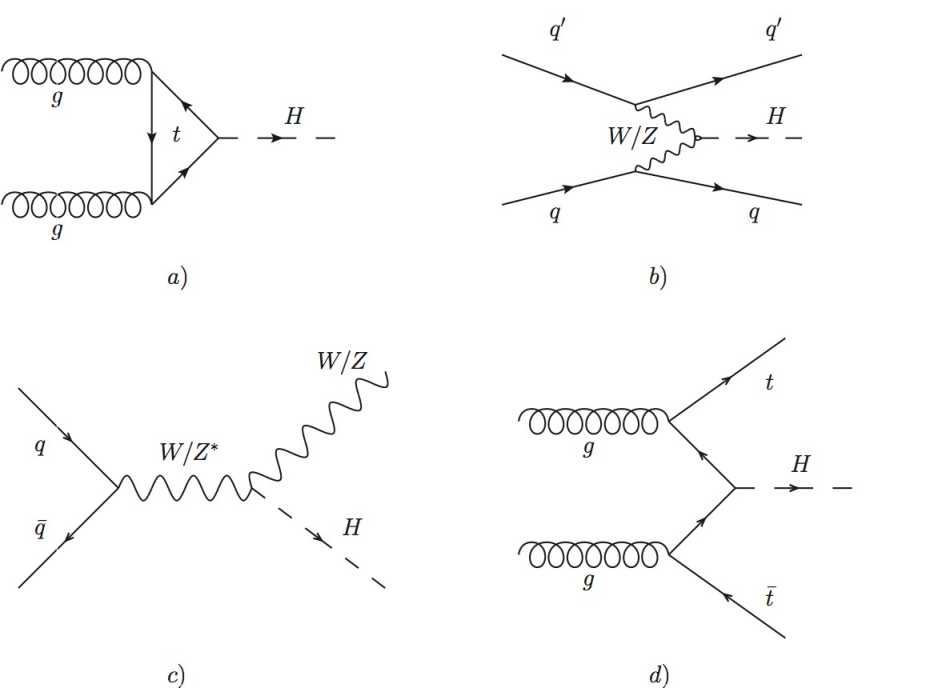
\includegraphics[width=0.8\textwidth]{chapter2/Higgs_production.jpg}
\caption{Production models in LHC}% \cite{Higgs_production_mode}}
\label{fig:SM_H_production}
\end{figure}









\section{Lepton flavour violation in beyond stand model theories}
Lepton flavour violating Higgs decays are forbidden in SM. The specific terms will not be compatible with renormalization. But beyond Standard Model, Lepton flavour conservation does not necessarily hold. In the following, two methods that can have lepton flavour violation are introduced, one model independent effective field approach and one with two Higgs doublet model. In both case, the focus is LFV Higgs decays and to show how LFV Higgs decays shows up in the new theories. 


\subsection{Lepton flavour violation Higgs decay in effective field theory}\label{effective_field}
The Effective Lagrangian approach is widely used to explore the new physics with higher dimensional operators in a model independent way. The Lagrangian in the theory can be written as following up to dimension six: 
\begin{equation}
L_{eff}=L_{SM}+\sum\frac{a^{ij}_{n}}{\Lambda^{2}}O^{ij}_{n}
\end{equation}
where $a^{ij}_{n}$ is the coefficients, $i,j,(=1,2,3)$ are flavour indices, n holds the number of the operators and $\Lambda$ is the new physics scale. 

There are various operators that can introduce processes that violate lepton flavour conservation~\cite{PhysRevD.62.116005}. As an example that most relevant to LFV Higgs decays, Yukawa-type operators that generate LFV Higgs decays only will be discussed. The Yukawa-type operators hold the following terms:
\begin{equation}
O^{ij}_{L\phi}=(\Phi^{\dagger}\Phi)(\bar{L}_{L_{i}}l_{R_{j}}\Phi)
\end{equation}
While, inside the Lagrangian, the change to SM Lagrangian takes the form:
\begin{equation}
\Delta L_{Y}=-\frac{\lambda^{'}_{ij}}{\Lambda^{2}}(\Phi^{\dagger}\Phi)(\bar{L}^{i}_{L}l^{j}_{R}\Phi)+h.c...
\end{equation}
Taking in the scalar doublet expansion around vev as shown in Equation.~\ref{Higgs_vev_expansion}, the O(6) Yukawa-type operators have the following form:
\begin{equation}
\begin{aligned}
\Delta L_{Y}=&-\frac{\lambda^{'}_{ij}}{\Lambda^{2}}(\Phi^{\dagger}\Phi)(\bar{L}^{i}_{L}l^{j}_{R}\Phi)+h.c...\\
         =&-\frac{\lambda^{'}_{ij}}{2\sqrt{2}\Lambda^{2}}l_{L}^{i}l_{R}^{j}(v+H)^{3}+h.c...\\
         =&-\frac{\lambda^{'}_{ij}v^{3}}{2\sqrt{2}\Lambda^{2}}l_{L}^{i}l_{R}^{j}-\frac{\lambda^{'}_{ij}3v^{2}}{2\sqrt{2}\Lambda^{2}}l_{L}^{i}l_{R}^{j}+h.c...
\end{aligned}
\end{equation}
The new Yukawa coupling terms have effects on fermion masses and SM Yukawa interactions. The SM components in Equation.~\ref{Higgsmuonmass} is obtained through the diagonalization of mass matrices~\cite{Harnik:2012pb}. The total Lagrangian is a combination of SM Lagrangian $L_{SM}$ and the effective field Lagrangian $\Delta L_{Y}$. Thus the combined fermion mass and Yukawa interaction terms are following:
\begin{equation}
\sqrt{2}m=V_{L}\Big[\lambda+\frac{v^{2}}{2\Lambda^{2}}\lambda^{'}\Big]V^{\dagger}_{R},~~\sqrt{2}Y=V_{L}\Big[\lambda+3\frac{v^{2}}{2\Lambda^{2}}\lambda^{'}\Big]V^{\dagger}_{R}
\end{equation}
The Yukawa couplings of Higgs and leptons mixed in the contributions from dimension six operators and have the following form, in which $\hat{\lambda=V_{L}\lambda^{'}V_{R}}$
\begin{equation}
Y_{ij}=\frac{m_{i}}{v}\delta_{ij}+\frac{v^{2}}{\sqrt{2}\Lambda^{2}}\hat{\lambda}_{ij}
\end{equation}
In the limit $\Lambda \to \infty$, the SM results can be recovered, but in general case, like in the electro-weak scale and a arbitrary non-diagonal matrix $\hat{\lambda}$, LFV Higgs decays can be introduced into the theory through effective fields.




\subsection{LFV in two Higgs models}

In the model with two Higgs doublets(2HDM) $\Phi_{1}$ and $\Phi_{2}$, similar to the SM, the Yukawa interaction can be written as: 
\begin{equation}
L=y_{1}\bar{L}\Phi_{1}E+y_{2}\bar{L}\Phi_{2}E+h.c,
\end{equation}
Here, $y_{1}$ and $y_{2}$ are Yukawa couplings. If there is not a parity symmetry distinguish the two Higgs doublets, there can be coupling of the two doublets to the leptons in the tree level. In general it is impossible to diagonalize $y_{1}$ and $y_{2}$ simultaneously and the LFV Higgs decay can be presented in the renormalizable Lagrangian~\cite{deLima2015}. A bit more description of 2HDM is in the following~\cite{BRANCO20121}.   


In 2HDM, there are in general four sub-type of models, the main difference comes from the coupling of Higgs doublets to the quarks and leptons as shown in Table.~\ref{2HDM_models}.
\begin{table}[htp!]
\caption{Four types of 2HDM models differs by the coupling to Higgs doublet fields}
\begin{center}
\begin{tabular}{|c|c|c|c|}
\hline
Model                                 &~  $u^{i}_{R}$~  &~  $d^{i}_{R}$ ~   &~   $e^{i}_{R}$ ~\\\hline
Type I                                 &  $\Phi_{2}$    &  $\Phi_{2}$     &  $\Phi_{2}$   \\\hline
Type II                                &  $\Phi_{2}$    &  $\Phi_{1}$     &  $\Phi_{1}$   \\\hline
Type III (lepton specific)     &  $\Phi_{2}$    &  $\Phi_{2}$     &  $\Phi_{1}$   \\\hline
Type IV (Flipped)                &  $\Phi_{2}$    &  $\Phi_{1}$     &  $\Phi_{2}$   \\\hline
\end{tabular}
\end{center}
\label{2HDM_models}
\end{table}
The type III 2HDM is more relevant to LFV which can have the tree level LFV Higgs decay. The Higgs doublets can have the general form:
\begin{equation}
\Phi_{j}=
\begin{pmatrix}
\phi^{+}_{j}    \\
(v_{j}+\phi_{j}+i\eta_{j}/\sqrt{2})
\end{pmatrix}
\end{equation}
Under the common assumption of CP conservation in the Higgs sector and not spontaneously broken, the quartic odd terms are eliminated in the potential, then the scalar potential can be expressed as
\begin{equation}
\begin{aligned}
V=&m^{2}_{11}\Phi^{\dagger}_{1}\Phi_{1}+m^{2}_{22}\Phi^{\dagger}_{2}\Phi_{2}-m^{2}_{12}(\Phi^{\dagger}_{1}\Phi_{2}+\Phi^{\dagger}_{2}\Phi_{1})+\frac{\lambda_{1}}{2}(\Phi^{\dagger}_{1}\Phi_{1})^{2}+\\
  &\frac{\lambda_{2}}{2}(\Phi^{\dagger}_{2}\Phi_{2})^{2}+\lambda_{3}\Phi^{\dagger}_{1}\Phi_{1}\Phi^{\dagger}_{2}\Phi_{2}+\lambda_{4}\Phi^{\dagger}_{1}\Phi_{2}\Phi^{\dagger}_{2}\Phi_{1}+\frac{\lambda_{5}}{2}[(\Phi^{\dagger}_{1}\Phi_{2})^{2}+(\Phi^{\dagger}_{2}\Phi_{1})^{2}]
  \end{aligned}
\end{equation}
The scalar doublets fields $\Phi_{1}$ and $\Phi_{2}$ are not physical observables but the mass eigenstates. So any combination of the scalar doublet fields, as long as it preserve CP and solid gauge symmetries in SM, produces the same physics results~\cite{BRANCO20121}. The following based is referred as Higgs basis for the Higgs doublets:
\begin{equation}\label{Higgs_base}
H_{1}=
\begin{pmatrix}
G^{+}    \\
\frac{1}{\sqrt(2)}(v+\phi^{0}_{1}+iG^{0})
\end{pmatrix}~,~
H_{2}=
\begin{pmatrix}
H^{+}    \\
\frac{1}{\sqrt(2)}(\phi^{0}_{2}+iA)
\end{pmatrix}
\end{equation}
The relationship between scalar field $\rho_{1}$ and $\rho_{2}$ and Higgs mass eigenstates h and H is the following:
\begin{equation}\label{Higgs_mass_states}
\begin{aligned}
h=&sin(\alpha-\beta)\phi_{1}^{0}+cos(\alpha-\beta)\phi_{2}^{0}\\
H=&cos(\alpha-\beta)\phi_{1}^{0}-sin(\alpha-\beta)\phi_{2}^{0}
\end{aligned}
\end{equation}
The angle $\alpha-\beta$ is the mixing angle between these two groups of scalars. The interactions of Higgs and fermions are through Yukawa coupling. In the Higgs base, the Yukawa interaction terms in the Lagrangian of the 2HDM can be expressed as:
\begin{equation}
\begin{aligned}
-L_{Y}=&\sqrt{2}\big(\bar{q}_{L_{j}}\tilde{H}_{1}\frac{K^{\ast}_{ij}m^{U}_{i}}{v}u_{R_{i}}+\bar{q}_{L_{i}}H_{1}\frac{m^{D}_{i}}{v}d_{R_{i}}+\bar{l}_{L_{i}}H_{1}\frac{m^{E}_{i}}{v}e_{R_{i}}\big) \\
            &+\bar{q}_{L_{i}}\tilde{H}_{2}\rho^{U}_{ij}u_{R_{j}}+\bar{q}_{L_{i}}H_{2}\rho^{D}_{ij}d_{R_{j}}+\bar{l}_{L_{i}}H_{2}\rho^{E}_{ij}e_{R_{j}}+h.c..
\end{aligned}
\end{equation}
Inside the Lagrangian, the terms denote as following, $\tilde{H}_i=i\sigma_{2}H^{\ast_{i}}$,  $K_{ij}$ as the CKM matrix and $\rho^{U,D,E}$ are complex matrices in flavor space. Taking in Equation.~\ref{Higgs_base} and \ref{Higgs_mass_states}, the lepton Yukawa interaction terms are collected as:
\begin{equation}
\begin{aligned}
-L_{Y}=&\bar{e}_{i}\big(\frac{m^{E}_{i}}{v}\delta_{ij}s_{\beta-\alpha}+\frac{1}{\sqrt{2}}\rho^{E}_{ij}c_{\beta-\alpha}\big)e_{j}h\\
            &+\bar{e}_{i}\big(\frac{m^{E}_{i}}{v}\delta_{ij}c_{\beta-\alpha}-\frac{1}{\sqrt{2}}\rho^{E}_{ij}S_{\beta-\alpha}\big)e_{j}H+...
\end{aligned}
\end{equation}
Term $s_{\beta-\alpha}$ and $c_{\beta-\alpha}$ stand for $sin_{\beta-\alpha}$ and $cos_{\beta-\alpha}$ respectively. The coupling of leptons and Higgs in the 2HDM model typeIII are expressed as
\begin{equation}
\begin{aligned}
g_{hff^{'}}&=\frac{m_{f}}{v}s_{\beta-\alpha}\delta_{ff^{'}}+\frac{\rho_{ff^{'}}}{\sqrt{2}}c_{\beta-\alpha}\\
g_{Hff^{'}}&=\frac{m_{f}}{v}s_{\beta-\alpha}\delta_{ff^{'}}-\frac{\rho_{ff^{'}}}{\sqrt{2}}c_{\beta-\alpha}\\
\end{aligned}
\end{equation}
So this shows the possibility of LFV Higgs decay at tree level~\cite{PhysRevD.90.115004}.








